% 6. Pruebas
\begin{frame}{Pruebas: validación de gramática}
  Validación coherente de símbolos, producciones y símbolo inicial.
  \vspace{2mm}
  \begin{center}
    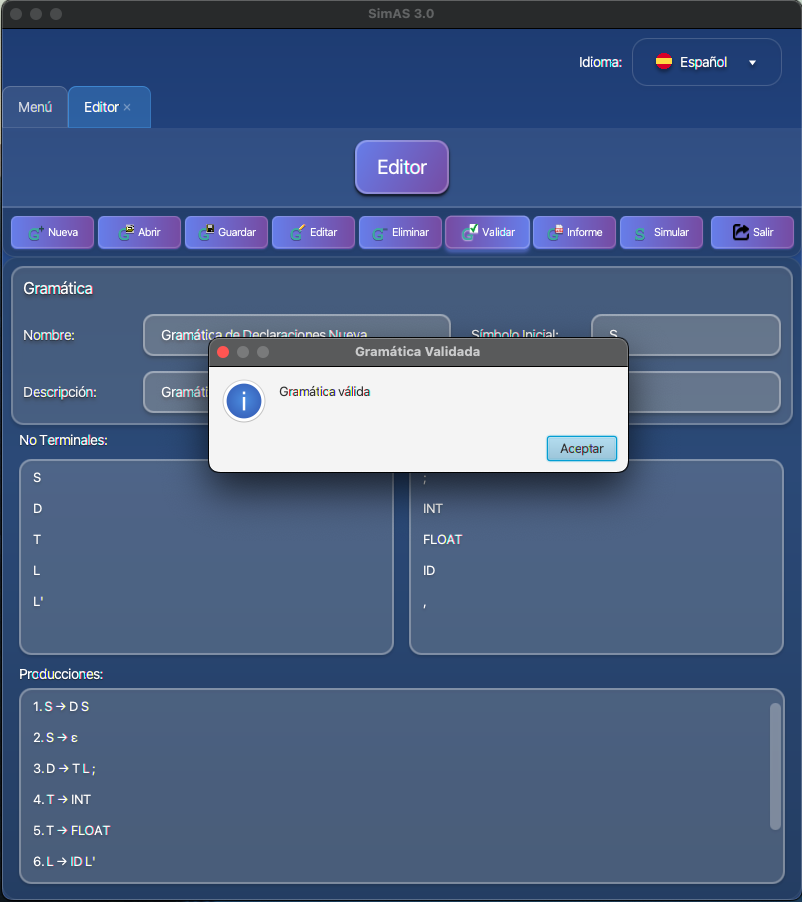
\includegraphics[width=0.98\linewidth,height=0.7\textheight,keepaspectratio]{../TFG_Antonio_Llamas_Garcia__SimAS_3_0____Manual_de_Usuario/figuras/editor/validar.png}
  \end{center}
\end{frame}

\begin{frame}{Pruebas: recursividad y factorización}
  Eliminación de recursividad izquierda y factorización correctas.
  \vspace{2mm}
  \begin{center}
    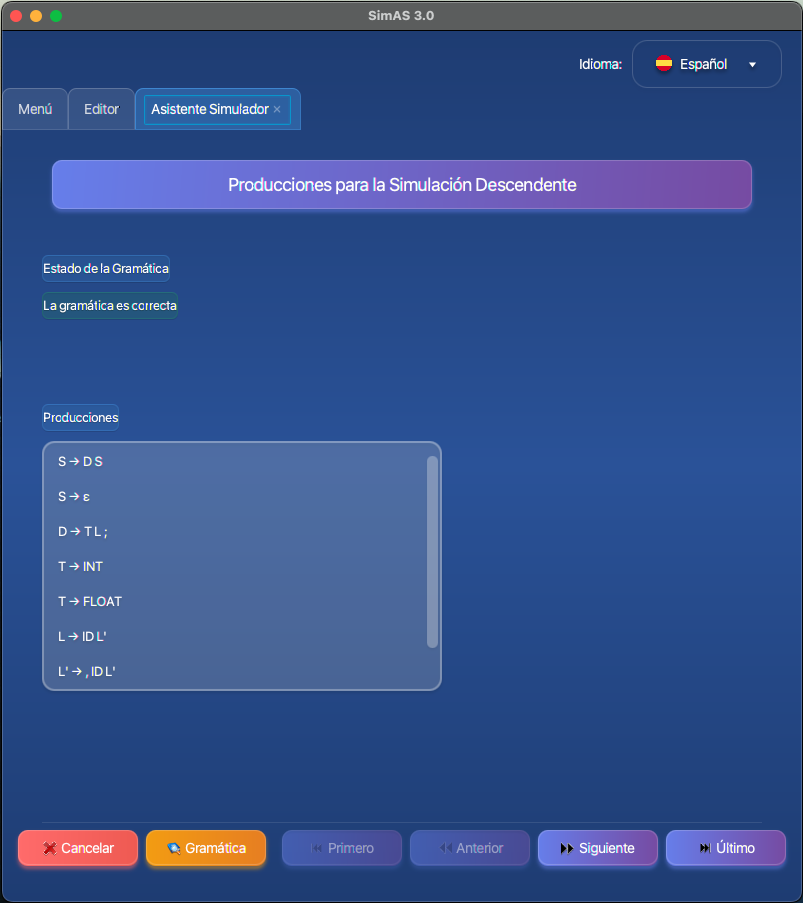
\includegraphics[width=0.98\linewidth,height=0.7\textheight,keepaspectratio]{../TFG_Antonio_Llamas_Garcia__SimAS_3_0____Manual_de_Usuario/figuras/simulador/paso1_recursividad_factorizacion.png}
  \end{center}
\end{frame}

\begin{frame}{Pruebas: conjuntos Primero/Siguiente}
  Cálculo estable y correcto de los conjuntos Primero/Siguiente.
  \vspace{2mm}
  \begin{center}
    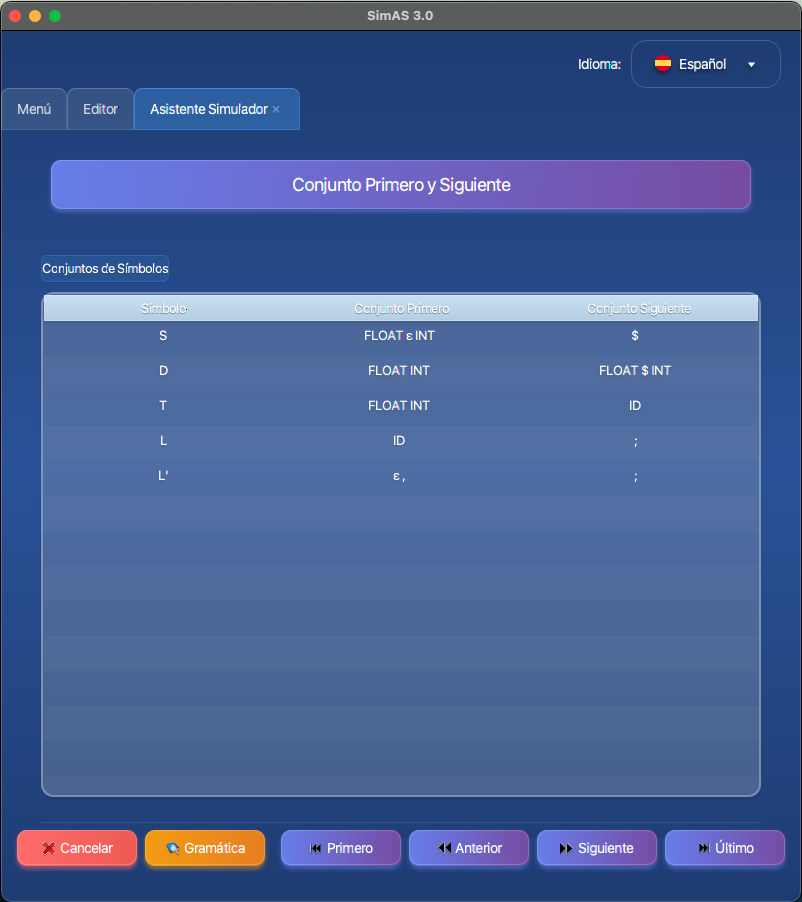
\includegraphics[width=0.98\linewidth,height=0.7\textheight,keepaspectratio]{../TFG_Antonio_Llamas_Garcia__SimAS_3_0____Manual_de_Usuario/figuras/simulador/paso2_conjuntos.png}
  \end{center}
\end{frame}

\begin{frame}{Pruebas: tabla predictiva LL(1)}
  Construcción de la tabla predictiva LL(1) sin ambigüedades.
  \vspace{2mm}
  \begin{center}
    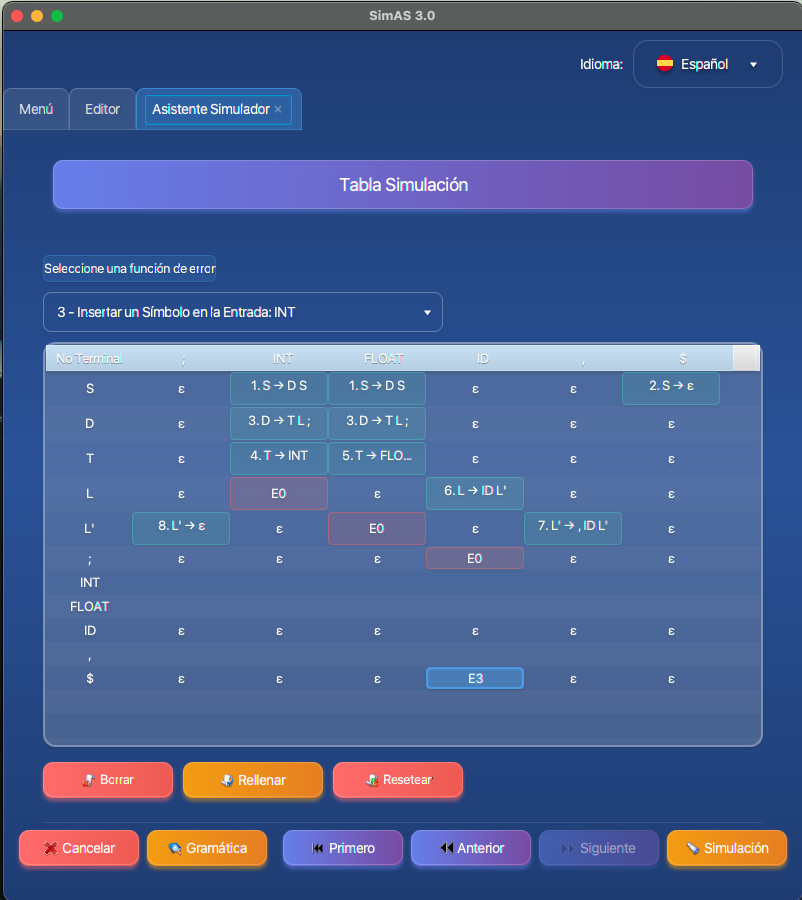
\includegraphics[width=0.98\linewidth,height=0.7\textheight,keepaspectratio]{../TFG_Antonio_Llamas_Garcia__SimAS_3_0____Manual_de_Usuario/figuras/simulador/paso5_tablaPredictivaCompleta.png}
  \end{center}
\end{frame}

\begin{frame}{Pruebas: funciones de recuperación de errores}
  Integración de funciones de error en la construcción y simulación.
  \vspace{2mm}
  \begin{center}
    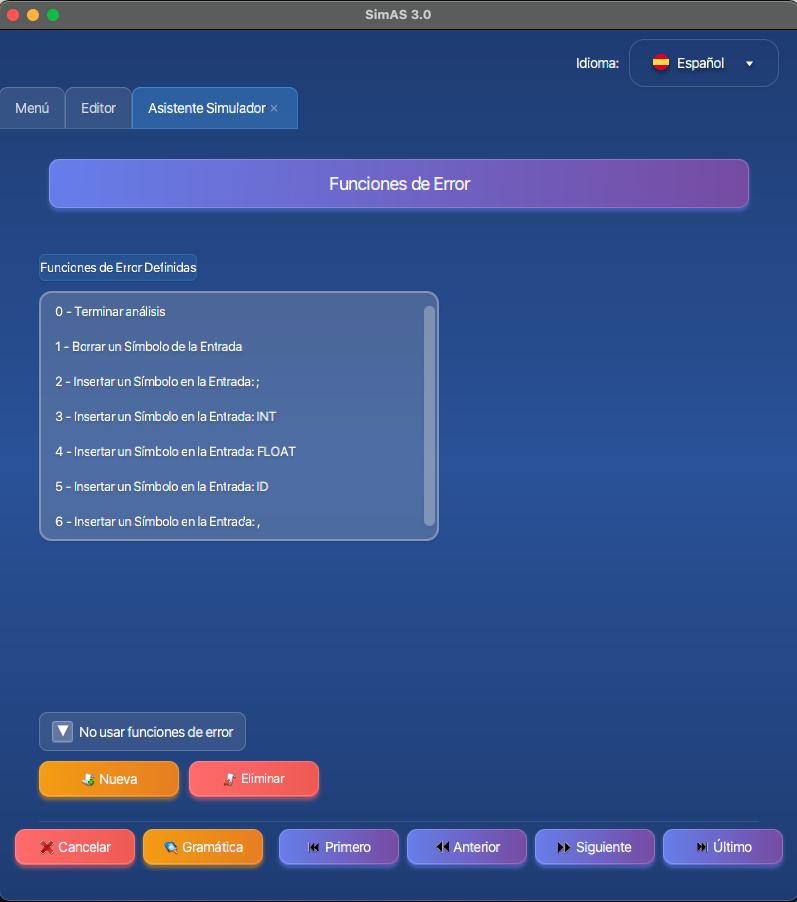
\includegraphics[width=0.98\linewidth,height=0.7\textheight,keepaspectratio]{../TFG_Antonio_Llamas_Garcia__SimAS_3_0____Manual_de_Usuario/figuras/simulador/paso4_funcionesError.png}
  \end{center}
\end{frame}

\begin{frame}{Pruebas: derivación paso a paso}
  Simulación determinista de la derivación de la cadena.
  \vspace{2mm}
  \begin{center}
    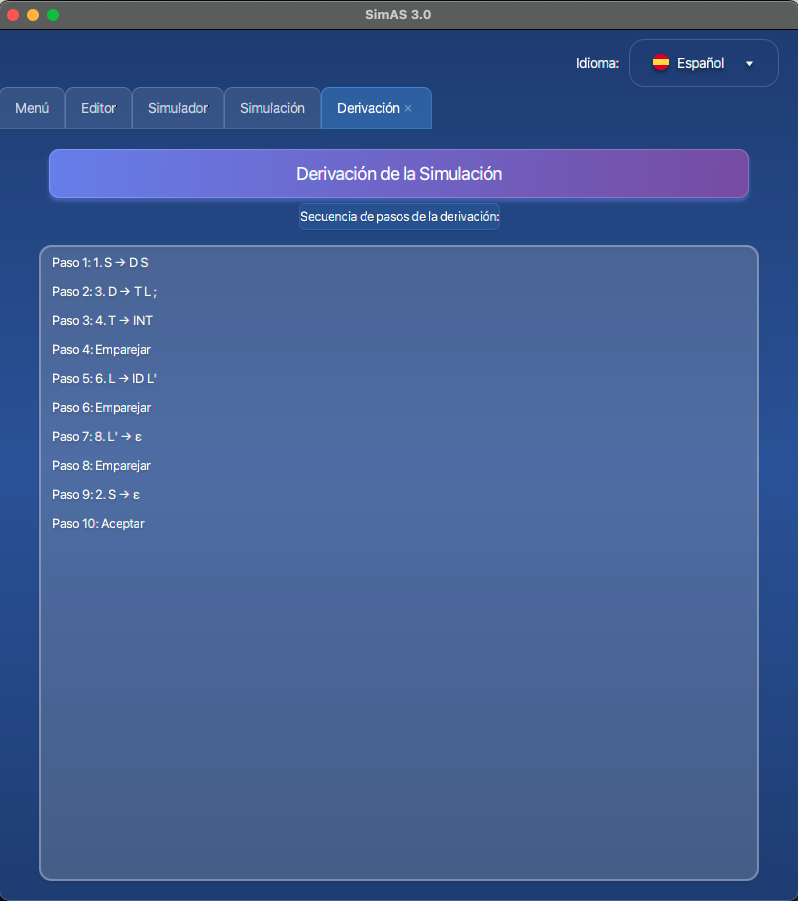
\includegraphics[width=0.98\linewidth,height=0.7\textheight,keepaspectratio]{../TFG_Antonio_Llamas_Garcia__SimAS_3_0____Manual_de_Usuario/figuras/simulador/simulacion_derivacion.png}
  \end{center}
\end{frame}

\begin{frame}{Pruebas: árbol sintáctico}
  Construcción del árbol sintáctico consistente con la derivación.
  \vspace{2mm}
  \begin{center}
    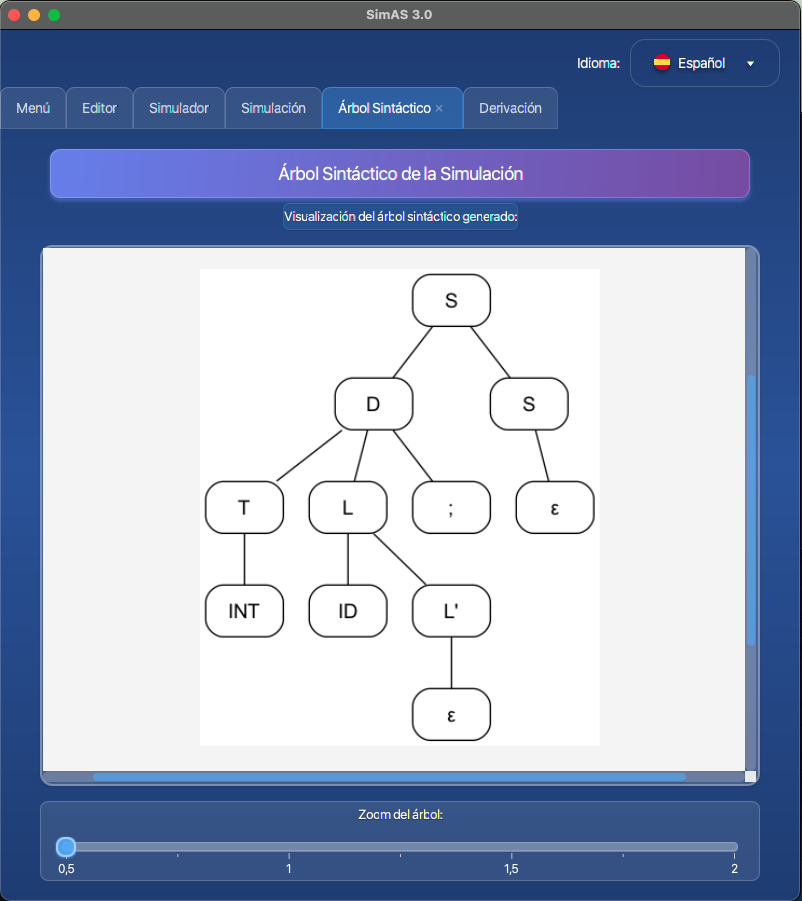
\includegraphics[width=0.98\linewidth,height=0.7\textheight,keepaspectratio]{../TFG_Antonio_Llamas_Garcia__SimAS_3_0____Manual_de_Usuario/figuras/simulador/simulacion_arbol.png}
  \end{center}
\end{frame}


